\documentclass{beamer}
%\mode<presentation>{}
\usepackage{graphicx}
\usepackage{verbatim}
\usetheme{Warsaw}
\title{Introduction to Bucket Sort}
\author{Bishwajit Saha}
\institute{Dept. of CSE, BUET}
\date{5th International Workshop on Algorithms}
\titlegraphic{
\includegraphics[width=1.5cm]{BuetLogo.png}
}
\begin{document}
\AtBeginSection[]
{
\begin{frame}{Table of Contents}
\tableofcontents[currentsection]
\end{frame}
}
\begin{frame}
	\titlepage
\end{frame}

\begin{frame}
	\frametitle{Outline}
	\tableofcontents
\end{frame}
\section{Introduction}

\begin{frame}
	\frametitle{Introduction}
	\begin{itemize}
		\pause\item What is meant by bucket??.
		
	\end{itemize}
	\pause
	\begin{figure}
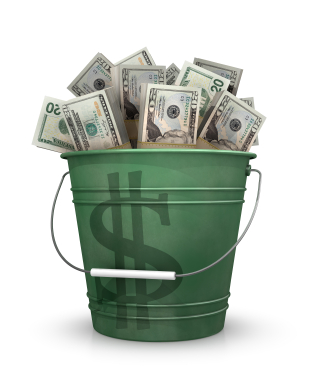
\includegraphics[scale=1.5]{bucket.png}
\caption{Bucket!!}
\end{figure}	
\end{frame}

\begin{frame}
	\frametitle{Introduction}
	What is bucket sort??
	\begin{itemize}
		\pause\item Distributes all the elements of an array into a number of buckets
		\pause\item Then each bucket is sorted individually
		\begin{itemize}
		\pause\item Either using a different sorting algorithm like insertion sort
		\pause\item Or by recursivly applying the bucket sort algorithm
		\end{itemize}
		\pause\item Also called Bin sort
		\pause\item Cousine of radix sort
		
	\end{itemize}
\end{frame}
\section{Working Strategy}

\begin{frame}
	\frametitle{Working Strategy}
	{\Large Pseudocode :}\\ 
	\textbf{function} bucketSort(array, n) \textbf{is}\\
	buckets $\leftarrow$ new array of n empty lists\\
	\textbf{for} i = 0 to (length(array)-1) \textbf{do}\\
	insert \emph{array[i]} into buckets[msbits(array[i], k)]\\
	 \textbf{for} i = 0 to n - 1 \textbf{do}\\
	 nextSort(buckets[i]);\\
  \textbf{return} the concatenation of buckets[0], ...., buckets[n-1]
\end{frame}  
  
  \begin{frame}
	\frametitle{Working Strategy}
  \begin{columns}
		\begin{column}{0.5\textwidth}

			\begin{itemize}
		\item Set up an array of initially empty "buckets"
		\pause\item \textbf{Scatter:} Go over the original array, putting each object in its bucket.
		\pause\item Sort each non-empty bucket.
		\pause\item \textbf{Gather:} Visit the buckets in order and put all elements back into the original array.
		
	\end{itemize}
		\end{column}
		\pause
		\begin{column}{0.5\textwidth}
			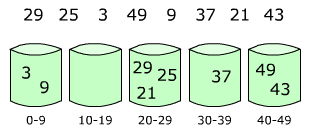
\includegraphics[width=1.1\columnwidth]{Bucket_sort_1.png}\\
			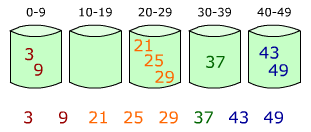
\includegraphics[width=1.1\columnwidth]{Bucket_sort_2.png}
		\end{column}
	\end{columns}
	
\end{frame}


\section{Variants}


\begin{frame}
	\frametitle{Conclusion}
	\begin{itemize}
	\item \textbf{Generic bucket sort}
	\item \textbf{ProxmapSort}
	\item \textbf{Histogram sort}
	\item \textbf{Postman's sort}
	\item \textbf{Shuffle sort}
	
	\end{itemize}
\end{frame}


\section{Optimization}
\begin{frame}
\begin{itemize}
\item A common optimization is :
\begin{itemize}
\pause\item put the unsorted elements of the buckets back in the original array first
\pause\item  then run insertion sort over the complete array
\end{itemize}
\pause\item insertion sort's runtime is based on how far each element is from its final position
\pause\item the number of comparisons remains relatively small
\end{itemize}
\end{frame}


\begin{frame}
Why we use this bucket sort??
\begin{itemize}
\pause\item Think about an array of 100000 elements!!
\pause\item If we use insertion sort algorithm to sort this array then we have to comapare almost 10000000000 times
\pause\item But if we use only 100 buckets to sort it then we have to compare only 100*(10000)=10000000 times
\pause\item It's here what this buckets give us advantages!!


\end{itemize}
\end{frame}
\end{document}
